\section{Study design}
\label{sec:study_design}
% Mention the build up of the chapter and the goal of the study.

This literature study has been designed and carried out by following 
well-accepted methodological guidelines on secondary studies, such as those in 
\cite{petersen2015guidelines_systematic, kitchenham2013systematic_review_guidelines, wohlin2012experimentation}.

This literature study researches multiple research questions. 
These questions will be given and motivated in subsection \ref{sec:study_design:research_questions}.
Then the search and selection of papers adhering to the inclusion and exclusion criteria began.
This process, and the criteria, are given in subsection \ref{sec:study_design:search_selection}.
After the selection was made final, these papers are hereon after called the \textit{primary studies}, the summarization and categorization process began. 
This process is the most important step for writing the literature study; the studies are made comparable by finding the commonalities and patterns in the field of study. 
This process is further explained in subsection \ref{sec:study_design:summ_categor}.


\subsection{Research Questions}
\label{sec:study_design:research_questions}
% Mention the research questions and their motivations (maybe metrics as well).
This study considers three research questions. These questions, their motivations and their metrics are given in this subsection.

\vspace{5mm}

\textbf{[RQ1]} \textit{What are the publication trends of papers on energy efficiency in robotics software?}

\vspace{5mm}

To be able to judge any characteristics of the state-of-the-art of energy efficiency in robotics software, we need to know the maturity of the field. What kind of publication trends are observed?

\vspace{5mm}

% \noindent\textbf{Metrics:} \textit{Publication Year} \\

\textbf{[RQ2]} \textit{What is the state-of-the-art on analyzing and improving the energy efficiency in robotics software?}

\vspace{5mm}

This research question aims to answer what the state-of-the-art is for achieving and analyzing an increase of energy efficiency in robotics software. It also aims to answer what the state-of-the-art is for uncovering aspects negatively impacting energy efficiency in robotics software.

\vspace{5mm}

% \noindent\textbf{Metrics:} \textit{Identified Major Consumer | Identified Improving (Software) Aspect | Major Contribution} \\

\textbf{[RQ3]} \textit{What are the trade-offs when dealing with energy efficiency in robotics software?}

\vspace{5mm}

This research question aims to give insights into what Quality Attributes have been identified to trade-off with energy efficiency. 
It is valuable for researchers and practitioners to know that if one wants to increase energy efficiency, one can expect a decrease of some other attribute.

% \noindent\textbf{Metrics:} \textit{QA Trade-offs} \\

\subsection{Search and Selection}
\label{sec:study_design:search_selection}
% Mention the search string CHECK, snowballing CHECK, criteria CHECK, duplicates CHECK, numbers from potentially relevant to primary CHECK.
% Mention how to filter potentially, not reading them all TODO. but checking all their titles TODO, reading those that seemed interesting. Abstract + full-text. Duplicates not in primary studies but read nonetheless CHECK.
\begin{figure}
    \centering
    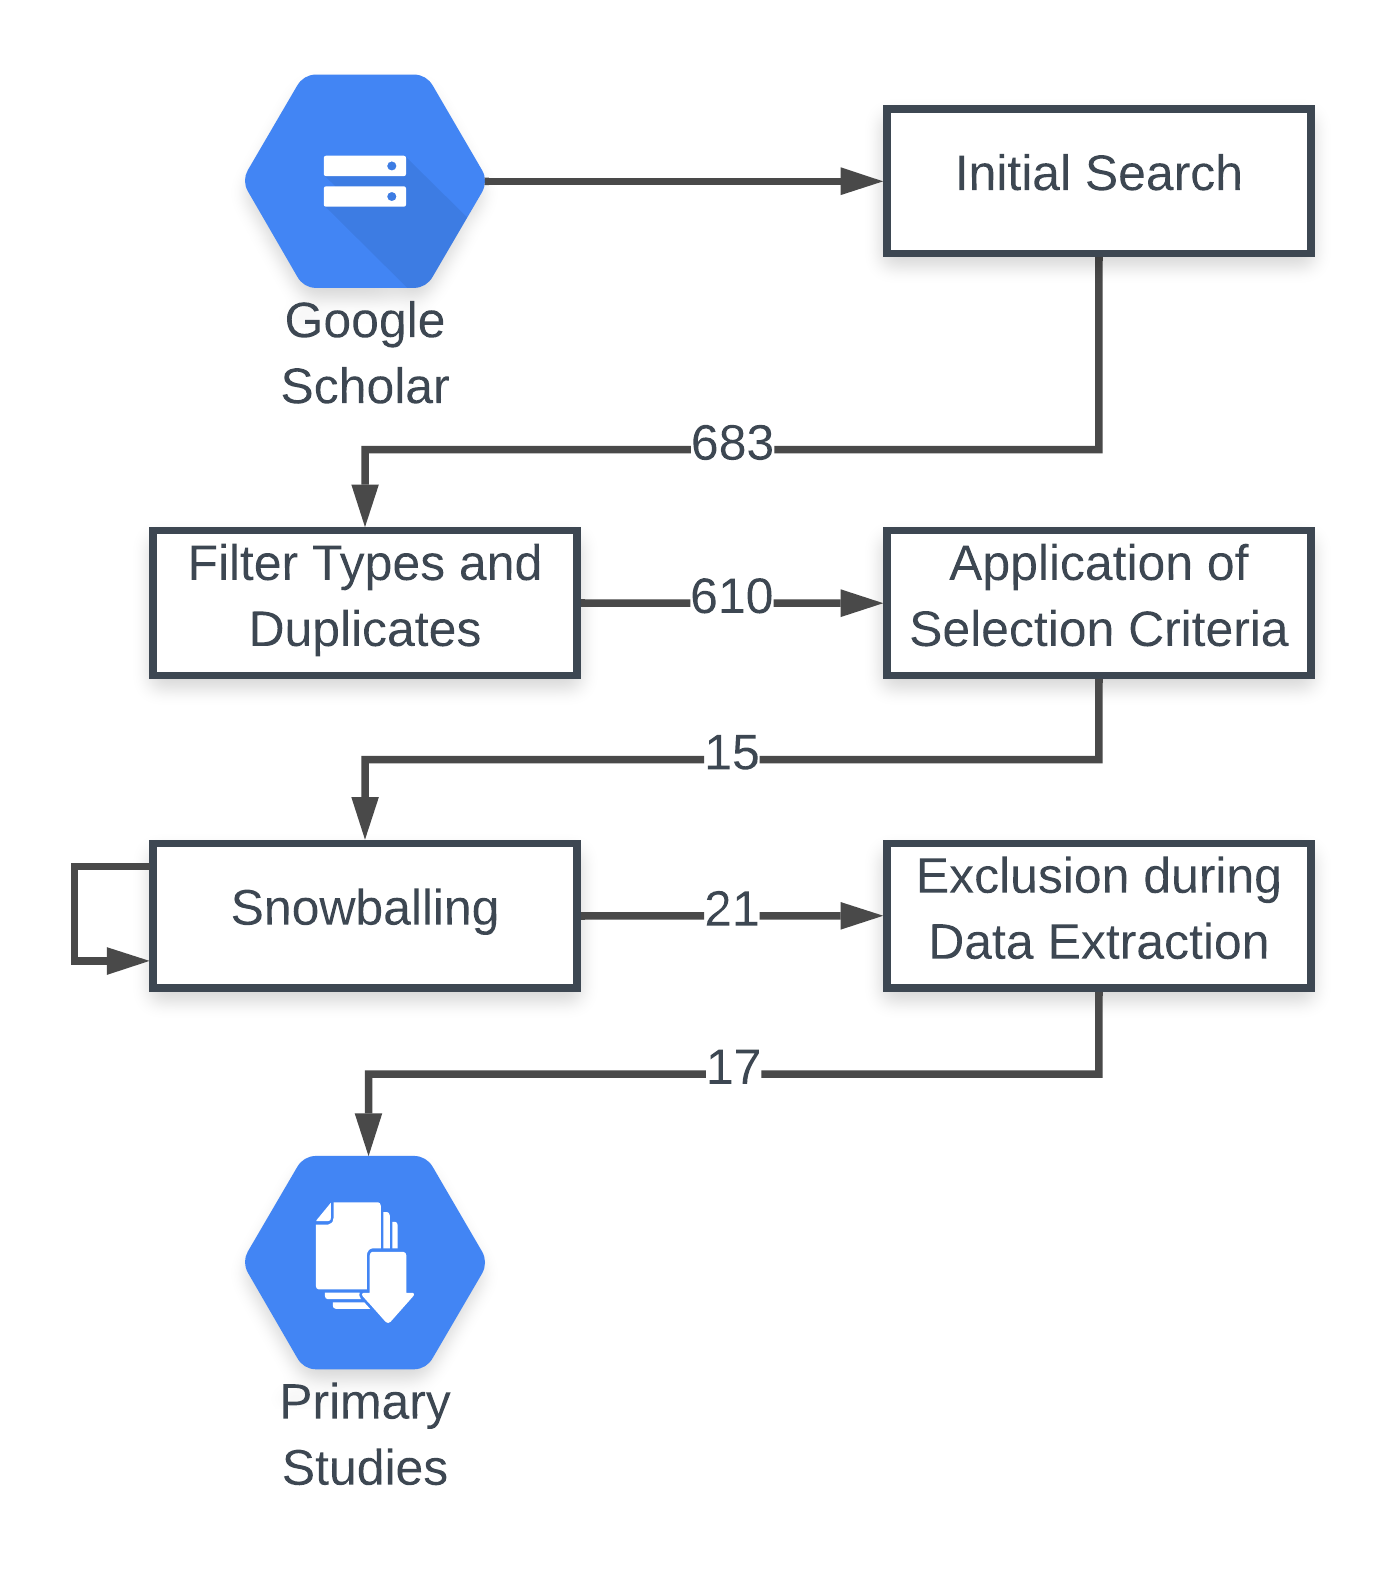
\includegraphics[width=0.5\textwidth]{figures/selection_process.png}
    \caption{The Search and Selection process}
    \label{fig:search_selec_process}
\end{figure}

After the familiarization process, the \textit{study design} is agreed and approved upon before starting the search and selection process. 
This is meant to prevent, as much as possible, any personal bias during search and selection, as the \textit{search string} and \textit{selection criteria} are already finalized.
An overview of the search and selection process is given in figure \ref{fig:search_selec_process}.
The process, as displayed in the figure, is further elaborated on in this subsection.

\vspace{5mm}

\noindent\textbf{1. Initial Search:}
For the initial search, \textbf{Google Scholar}\footnote{\url{https://scholar.google.com/}} was used. The results were retrieved using the \textit{search string} as given in figure \ref{fig:search_string}. 
The search string is kept as general as possible so that potentially relevant studies that would be able to make it to the primary studies but might not match exactly, are not accidentally filtered out by the crude, automatic search.
The number of results at the time of performing the initial search were \textbf{683} potentially relevant studies.

\begin{figure}
    \centering
    \textit{"(intitle:robot) AND (intitle:power OR intitle:green OR intitle:energy OR intitle:battery) AND software"}
    \caption{Search String}
    \label{fig:search_string}
\end{figure}

\noindent\textbf{2. Filter Types and Duplicates}
During this step, all publication types that are not peer-reviewed by nature are filtered out. 
The potentially relevant studies that resulted from the initial search were thus automatically filtered to be only of any of these types: \textit{Journal Articles, Conference Papers, Book Sections, Books}.
By filtering these types, the total number of potentially relevant studies went down to \textbf{615}. 
Then, the filtered collection was filtered automatically once more on explicit duplicates; duplicates that match in \textit{Title} and \textit{Author}.
In case a duplicate was found, meaning a paper was published in more than one instance (for example, if a conference paper was extended to a journal version), only one instance has been counted as a primary study. 
In those cases the journal version of the study has been preferred, as it is supposed to be the most complete; nevertheless, both versions have been used in the data extraction phase and in the analysis of the publication trends (RQ1, see section \ref{sec:results}).
After the duplicates were removed the total number of potentially relevant studies decreased to \textbf{610}.

\vspace{1mm}

\textit{\textbf{Note:} this step will only filter easy duplicates (fully matching Title and Authors sections) by design. Any other duplicate is left to be manually removed in order to prevent unintentional removal. See section \ref{sec:threats}}.

\vspace{5mm}

\noindent\textbf{3. Application of Selection Criteria:}
During this step the \textbf{610} potentially relevant studies are filtered by applying the selection criteria. 
The study is added to the set of \textit{primary studies} in case it adheres to \textbf{all} of the inclusion criteria (\textit{i1-i5}) and \textbf{none} of the exclusion criteria (\textit{e1-e5}). 
These criteria, in the context of \textit{Robotics Software}, consist of:
\begin{itemize}
	\item[i1] Studies focussing on energy efficiency.
    \item[i2] Studies focussing on software aspects.
    \item[i3] Studies providing evaluation.
    \item[i4] Studies that are peer-reviewed.
    \item[i5] Studies written in English.
    
	\item[e1] Studies that, while focussing on energy efficiency, do not explicitly deal with any software aspect.
    \item[e2] Studies where energy efficiency is only used as an example.
    \item[e3] Secondary or Tertiary studies (literature reviews, theses etc).
    \item[e4] Studies that are not in the form of a Journal Article, Conference Paper, Book or Book Section.
    \item[e5] Studies not available as full-text.
\end{itemize}

% Write that these were applied manually, reading titles, if not enough, reading abstract, if not enough, reading full-text.
The application of the selection criteria was done manually by following the steps given below. Each step was performed to see if any selection criteria could be decided based on the information gained by it. If a step decides one of the \textit{exclusion criteria} the next steps are not followed for that particular study, as it already warrants rejection. The following steps were followed for each of the \textbf{610} potentially relevant studies:
\begin{itemize}
	\item[S1] Read the \textit{Title}.
	\item[S2] \textit{Download} the study.
	\item[S3] Read the \textit{abstract}.
	\item[S4] Read the study \textit{full-text}.
\end{itemize}

After this step, a total of \textbf{15} papers were identified to adhere to \textbf{all} of the \textit{inclusion criteria} and \textbf{none} of the \textit{exclusion criteria}. These form the set of \textbf{considered studies}.

\vspace{5mm}

\noindent\textbf{4. Snowballing:}
In this phase the automatic search was complemented with recursive \textit{backward} and \textit{forward} snowballing \cite{wohlin2014snowballing}.
During the \textit{backward} snowballing, all references of each \textit{considered study} were added to the potentially relevant studies. 
After each reference from each considered study was added, the steps for applying the selection criteria, as given above, were once more followed. 
After completing this iteration, each newly considered study was also used in the recursive backward snowballing process.

Following the backward snowballing, \textit{forward} snowballing was used. 
In this process each study that cites each considered study is added to the potentially relevant studies, hereafter each step for applying the selection criteria was once more followed, and the newly considered studies were recursively used in the forward snowballing process.

\vspace{5mm}

On completion of the snowballing process, the set of considered studies grew to \textbf{21} studies. These studies now form the \textit{primary studies} set.

\vspace{5mm}

\noindent\textbf{5. Exclusion during Data Extraction:}
% Data sheet, extraction, warranting rejection if exclusion criteria are met.
During the data extraction phase, each \textit{primary study} if read full-text and its findings are used to construct a data sheet.
This data sheet aims to cover all similarities and patterns between the primary studies so that a report can be written, comparing their findings.
During this data extraction, papers that made it to the primary studies set can still be removed from the set if they are found to adhere to one of the \textit{exclusion criteria}.

The data sheet constructed during this phase, consists of a set of columns. 
These columns, example values and their most relevant RQ are given in table \ref{table:data_sheet}.

\begin{table*}[t]
    \centering
    \caption{Data sheet columns.}
    \begin{tabular}{llc}
        \toprule
            Column Name & 
            Example Value & 
            Relevant RQ  \\
        \midrule
            Date & 
                \textit{2020} & 
                RQ1 \\
            Energy Metric Used & 
                \textit{FPS / W (Watt)} & 
                RQ2 \\
            QA Trade-off presented & 
                \textit{Timeliness vs Efficiency} & 
                RQ3 \\
            Application Domain & 
                \textit{Robot Exploration} & 
                RQ2 \\
            Identified Major Consumers & 
                \textit{Too many stops and turns in path} & 
                RQ2 \\
            Identified (Software) Aspect Improving Efficiency & 
                \textit{Improved path finder} & 
                RQ2 \\
            Major Contribution & 
                \textit{The actual improved, evaluated, path finder algorithm} & 
                RQ2 \\
            Experiment & 
                \textit{None / Simulation / Real-World / Combination} & 
                RQ2 \\
            Comparison Against State-Of-The-Art & 
                \textit{Yes / No} & 
                RQ2 \\
            Energy Model Used &
                \textit{1 Unit of Distance = 1 Unit of Energy} & 
                RQ2 \\
        \bottomrule
    \end{tabular}
    \label{table:data_sheet}
\end{table*}

\subsection{Summarization and Categorization}
\label{sec:study_design:summ_categor}
% Add diagram displaying the summarization and categorization process (reading papers, taking notes, categorizing the similarities, building data sheet, reading papers again and filling in data sheet.)

Arriving at this step, the set of \textit{primary studies} is finalized, now consisting of \textbf{17} papers.
After reading all primary studies once more, their data sheets, as given in table \ref{table:data_sheet}, are filled in manually. 
Once the data sheet has been fully filled in, the report can be written. 
The results, as shown in section \ref{sec:results}, are based on this completed data sheet.